
\documentclass{beamer}
\usepackage[utf8]{inputenc}
\usepackage{amsfonts}
\usepackage{amsmath}
\usepackage{amssymb}
\usepackage{graphicx}

\usepackage{hyperref}
%_____________________  _____     _____  ____________________  
%\______   \_   _____/ /  _  \   /     \ \_   _____\______   \ 
% |    |  _/|    __)_ /  /_\  \ /  \ /  \ |    __)_ |       _/ 
% |    |   \|        /    |    /    Y    \|        \|    |   \ 
% |______  /_______  \____|__  \____|__  /_______  /|____|_  / 
%        \/        \/        \/        \/        \/        \/  
                                                              
\usetheme{Madrid}
\defbeamertemplate*{footline}{shadow theme}
{%
  \leavevmode%
  \hbox{\begin{beamercolorbox}[wd=.5\paperwidth,ht=2.5ex,dp=1.125ex,leftskip=.3cm plus1fil,rightskip=.3cm]{author in head/foot}%
    \usebeamerfont{author in head/foot}\insertframenumber\,/\,\inserttotalframenumber\hfill\insertshortauthor
  \end{beamercolorbox}%
  \begin{beamercolorbox}[wd=.5\paperwidth,ht=2.5ex,dp=1.125ex,leftskip=.3cm,rightskip=.3cm plus1fil]{title in head/foot}%
    \usebeamerfont{title in head/foot}\insertshorttitle%
  \end{beamercolorbox}}%
  \vskip0pt%
}

\title{\textit{Plum} para la construcción de modelos de edad}
\author{Dr. Marco Antonio Aquino López\\ CIMAT}
\date{\today}

\begin{document}
    \begin{frame}
    \maketitle
    \end{frame}

\begin{frame}{\textit{Plum} } 
	\begin{block}{\textit{Plum} }
		\begin{itemize}
			\item{ es un modelo bayesiano para el análisis de datos de $^{210}$Pb }
			\item{ separa el decaimiento del $^{210}$Pb y el modelo de edad}
			\item{ usa el modelo de edad Bacon para la estimación de la función edad-profundidad }
			\item{ permite la incorporación de información (otros fechamientos) de manera natural. }
		\end{itemize}
	\end{block}
\end{frame} 


\begin{frame}{\textit{rPlum}:Implementación de \textit{Plum} en R}
	\begin{block}{\textit{rPlum}}
		\begin{itemize}
			\item{ es un paquete en R para que implementación del modelo \textit{Plum}. }
			\item{ instalación}
			\item{ uso con datos de $^{210}$Pb (y $^{226}$Ra).}
			\item{ incorporación de otros métodos de fechado}
			\item{ rangos de sedimentación}
		\end{itemize}
	\end{block} 
\end{frame} 

\begin{frame}{Modelo \textit{CRS}}
	\begin{center}
		\begin{tabular}{p{7.51cm}p{2.51cm}}
			Este modelo asume una tasa constante de suministro de $^{210}$Pb al sedimento.

			Y usa la función de decaimiento para inferir la edad de manera directa. 

			Como resultado se tiene una función de edad profundidad logarítmica. 
			$$t(x) = \frac{1}{\lambda}\log\left( \frac{A_0}{A_x} \right)$$ Appleby \& Oldfield (1979) ; Robbins (1979)   
			& 
 			\begin{minipage}{0.85\textwidth}
				\includegraphics[width=2.5cm]{./Figures/Core_CRS.png} 
			\end{minipage}
		\end{tabular}
	\end{center}
\end{frame} 

\begin{frame}{Modelo \textit{Plum}}
	\begin{center}
		\begin{tabular}{p{7.51cm}p{2.51cm}}
			Por otro lado, {\itshape Plum} usa inferencia estadística para inferir el modelo de edad.

			Primero se define estadísticamente una muestra de $^{210}$Pb  de la siguiente forma; 
			$$y_i\sim \mathcal{N}\left(\mu_i^s +\mu_i^u ,\sigma_i \right)$$  
			& 
			\begin{minipage}{0.5\textwidth}
				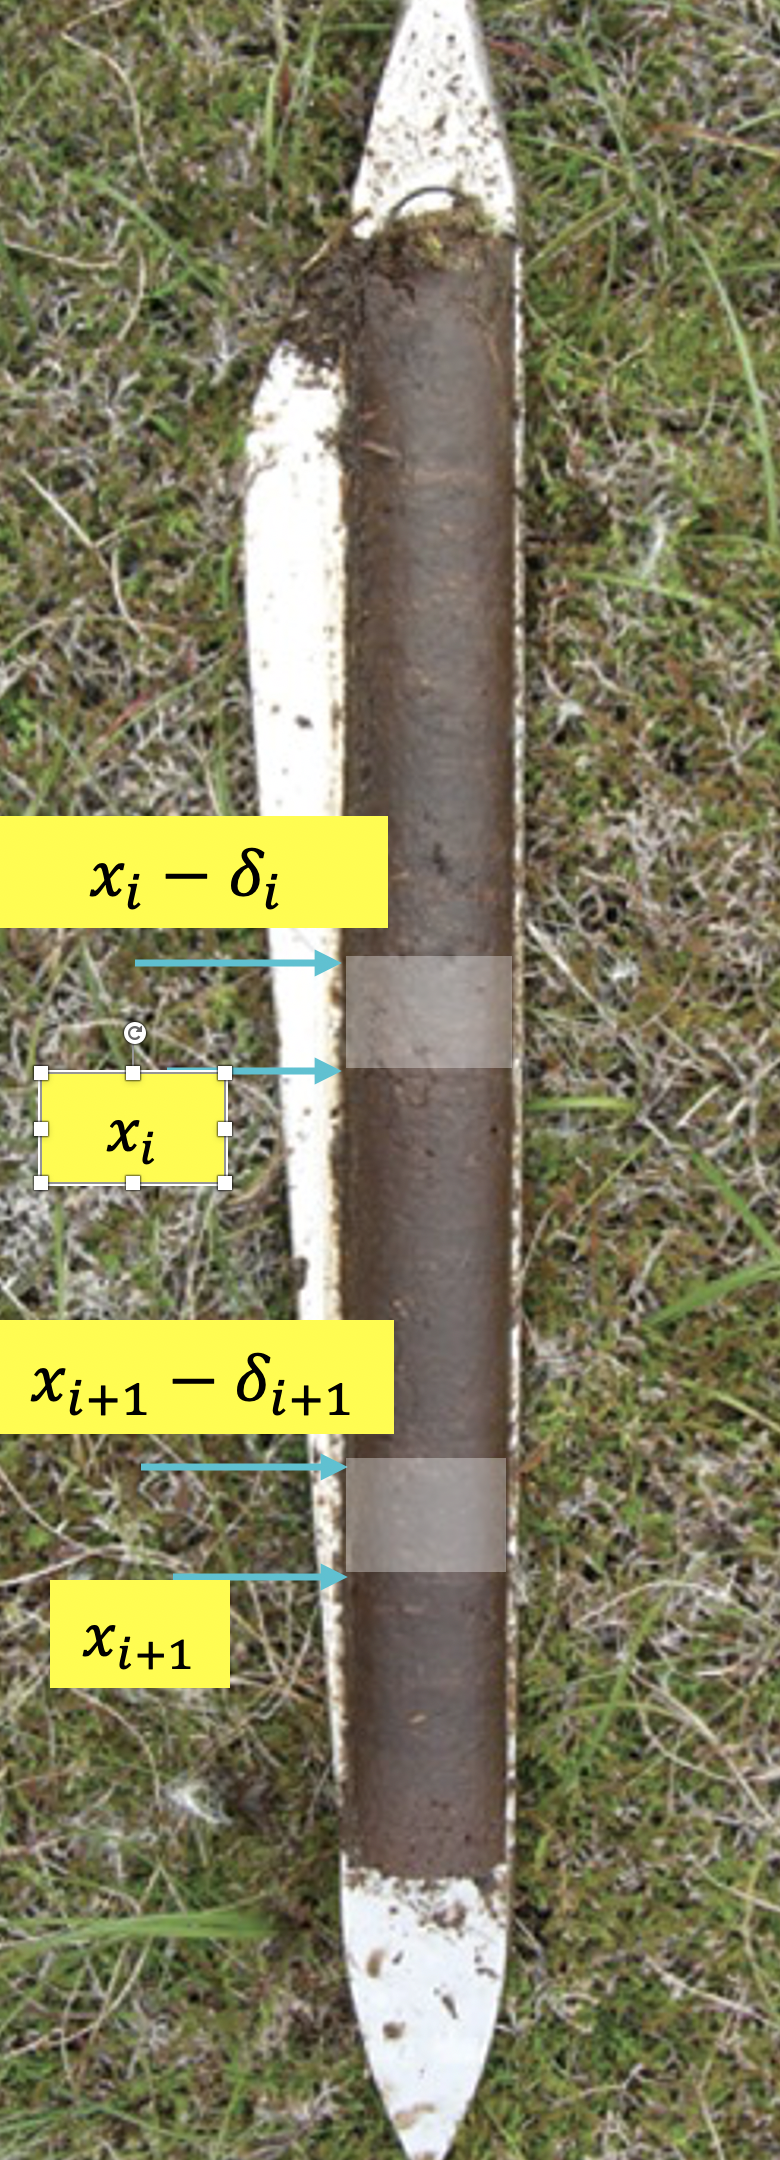
\includegraphics[width=2.5cm]{./Figures/Core_Plum.png} 
			\end{minipage}
		\end{tabular}
	\end{center}
\end{frame} 

\begin{frame}{Modelo \textit{Plum} }
	\begin{center}
		\begin{tabular}{p{7.51cm}p{2.51cm}}
			Sea $\mu_i^s$ el nivel "verdadero" $^{210}Pb$ soportado y $\mu_i^u$ el no soportado (exceso) en una muestra $y_i$. 

			Si asumimos un flujo constante de $^{210}Pb$ ($\Phi_i$) en muestra $y_i$, 
			$$\mu_i^u = \frac{\Phi_i}{\lambda} \left(e^{-\lambda t(x_i-\delta)}- e^{-\lambda t(x_i)} \right) $$ 	
			&
			\begin{minipage}{0.85\textwidth}
				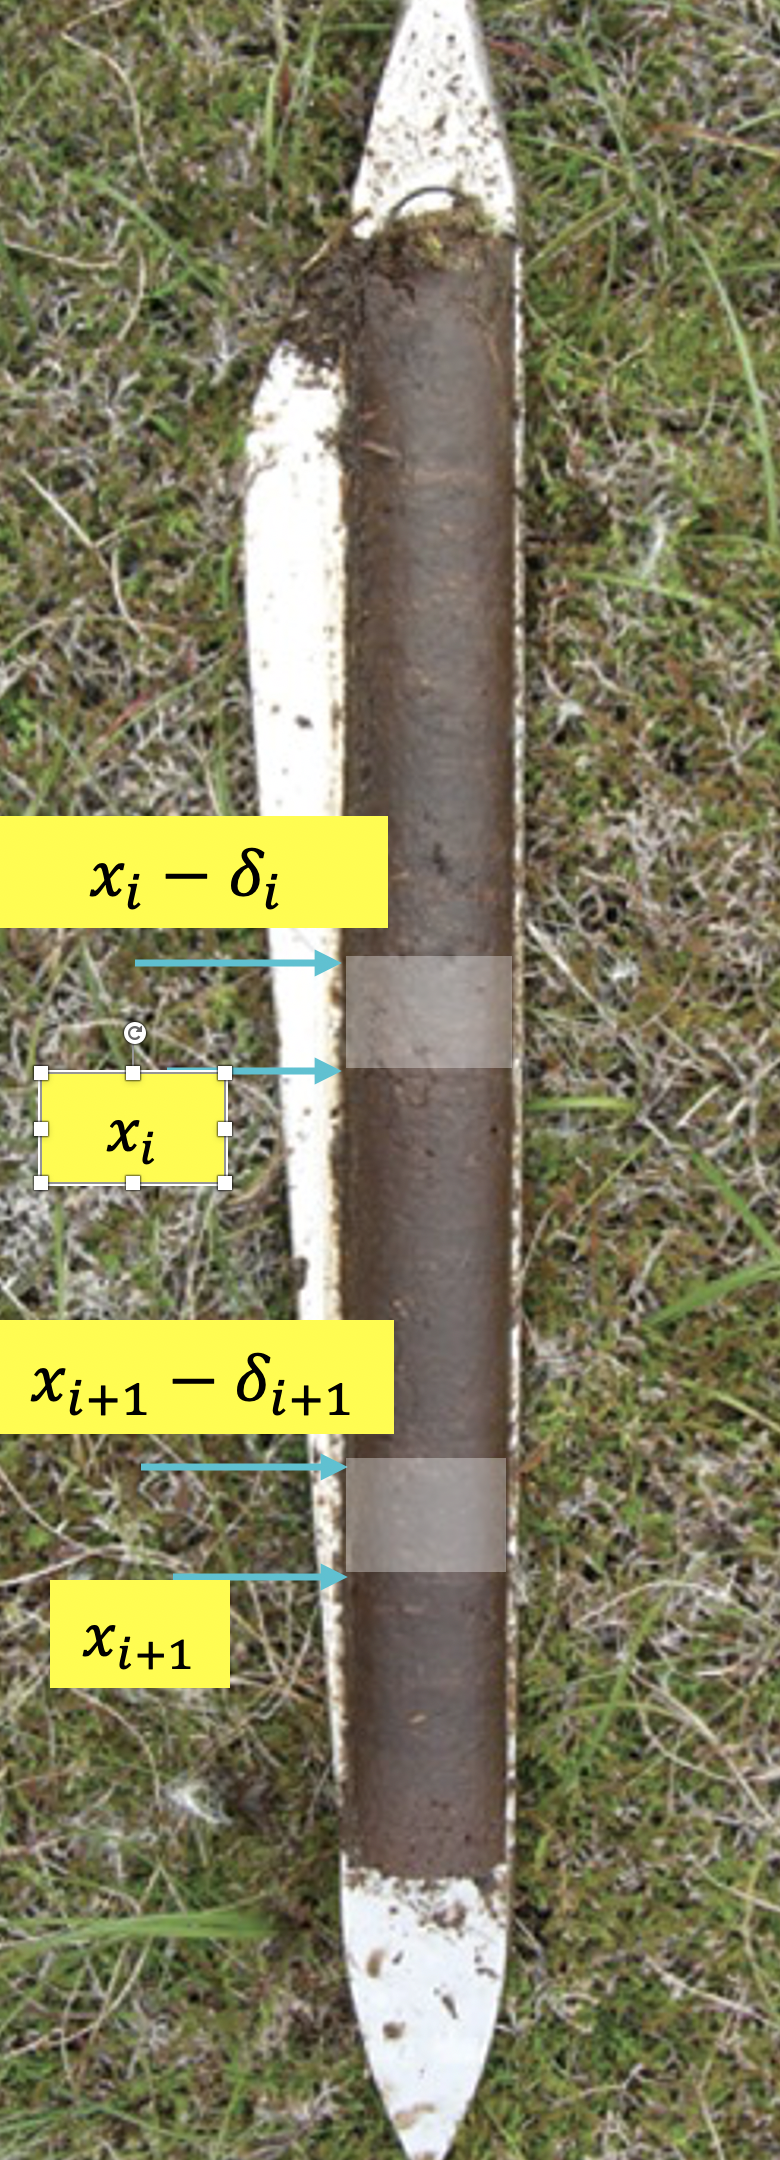
\includegraphics[width=2.5cm]{./Figures/Core_Plum.png} 
			\end{minipage}
		\end{tabular}
	\end{center}
\end{frame} 

\begin{frame}{Modelo de edad}
	\begin{block}{Modelo de edad \textit{Bacon} }
 		\begin{eqnarray}
			G(d,m) &=& \sum_{j=1}^i m_j \Delta c  + m_{i+1} (d-c_i)   , \nonumber \\
			m_j &=& \omega m_{j+1}+(1-\omega)\alpha_j \nonumber
		\end{eqnarray}
	\end{block} 
	\href{https://chrono.qub.ac.uk/blaauw/wiggles/Bayes.gif}{Animación provista por Dr. Blaauw}
\end{frame} 

\begin{frame}{Modelo \textit{Plum}}
	Con esto se puede definir la verosimilitud de manera adecuada.

	En esta ecuación el elemento de interés es la función de edad profundidad.
	\begin{block}{ Verosimilitud de \textit{Plum}}
 		\begin{eqnarray}
			y_i\mid P^S_i, \Phi_i, \bar{t} &\sim& \mathcal{N} \left(\mu^s_i+\frac{\Phi_i}{\lambda} \left( e^{-\lambda G(x_i-\delta_i)} - e^{-\lambda G(x_i)} \right), (\sigma_i\rho_i)^2 \right) \nonumber \\
			\ell(Y \mid P^S_i, \Phi_i, \bar{t}  ) &\propto&  -\sum_{i=1}^n \frac{\left(y_i-\left(A_i^S+ \frac{\Phi_i}{\lambda}\left( e^{-\lambda G(x_{i-1},m)} - e^{-\lambda G(x_{i},m)}\right) \right)\right)^2}{2\sigma_i^2} \nonumber \\
			& & - \sum_{j=1}^{n_s} \frac{(y_j^S-P^S)}{2\sigma_j^2} \nonumber
		\end{eqnarray}
	\end{block} 
	\end{frame} 



\begin{frame}{Distribuciones a priori }	
	\begin{block}{ }
 		\begin{itemize}
			\item{Actividad soportada: $$\mu_i^s \propto Gamma(2,1/10)$$ }
			\item{Flujo de 210Pb al sedimento:  $$\Phi\proto Gamma(2,1/25)$$}
			\item{Taza de acumulación: $$\alpha_i \propto Gamma(1.5,1.5/10)$$ }
			\item{Memoria: $$\omega_i \propto Beta(5,5)$$}
		\end{itemize}
	\end{block} 
	\textit{Note: En el caso del flujo de $^{210}$Pb para facilitar los cálculos y tiempos de computo se asume constante en toda la cronología. }
\end{frame} 

\begin{frame}{\textit{Plum} }
	La estructura de este modelo es compleja así que se hace uso de Markov Chain Monte Carlo.

	\href{https://www.researchgate.net/project/Plum-package}{Animación de \textit{Plum}}
\end{frame} 

\begin{frame}{\textit{Plum} }
		\begin{figure}
			\begin{centering}
				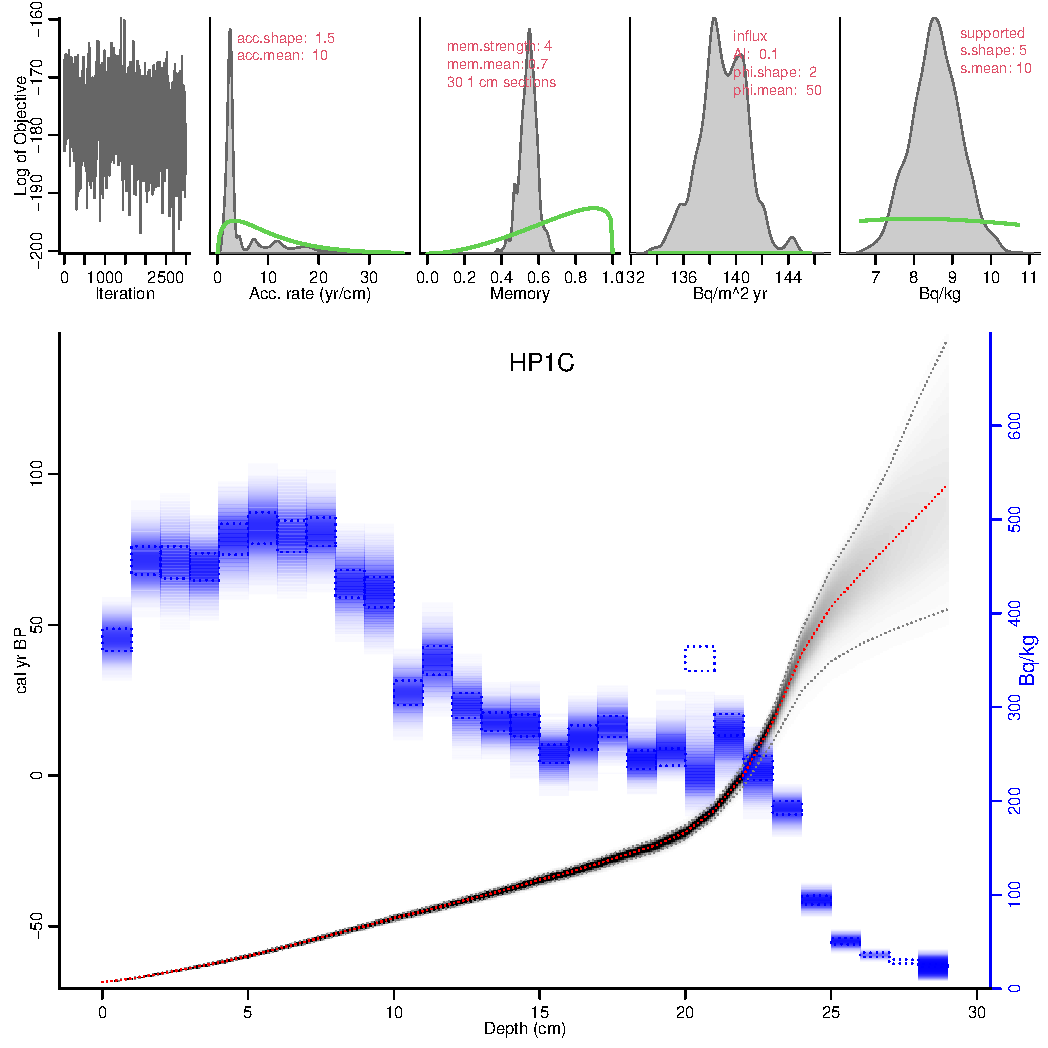
\includegraphics[width=8cm]{./Figures/HP1C_30.pdf}
				\caption{}
				\label{}
			\end{centering}
		\end{figure}
\end{frame} 

\begin{frame}{Aprendizaje (limite de edad)}
	\begin{figure}
		\begin{centering}
			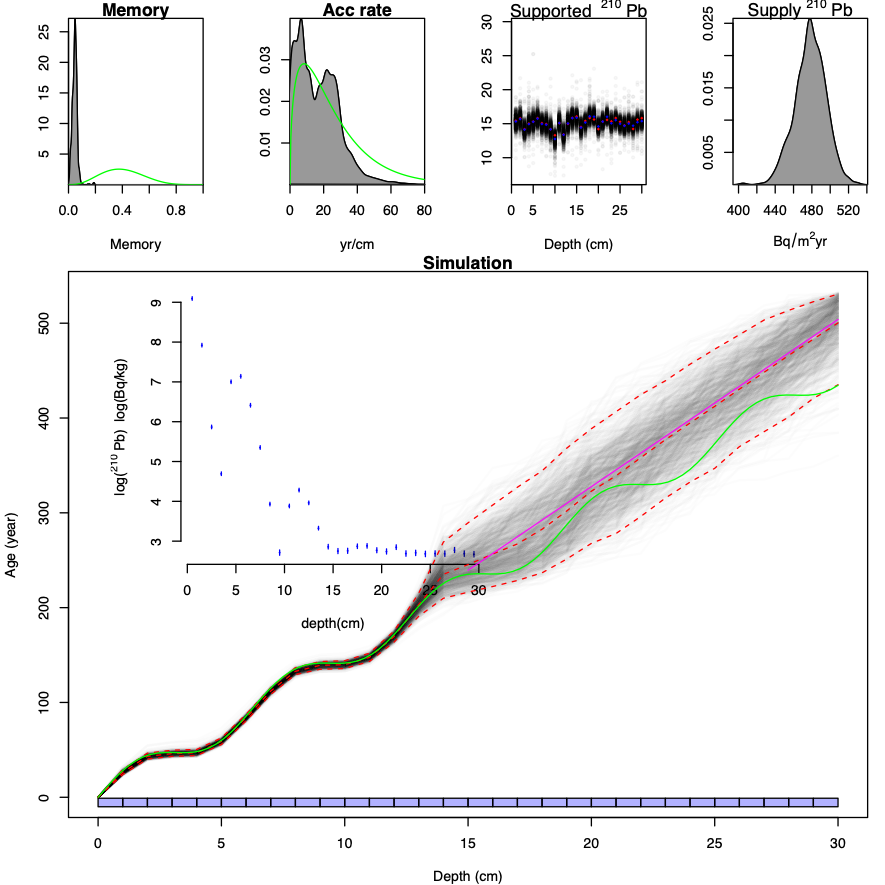
\includegraphics[width=8cm]{./Figures/Absurde_age_lim.png}
			\caption{}
			\label{}
		\end{centering}
	\end{figure}
\end{frame} 





\begin{frame}{Aprendizaje (muestreo)}
 	\begin{figure}
		\begin{centering}
			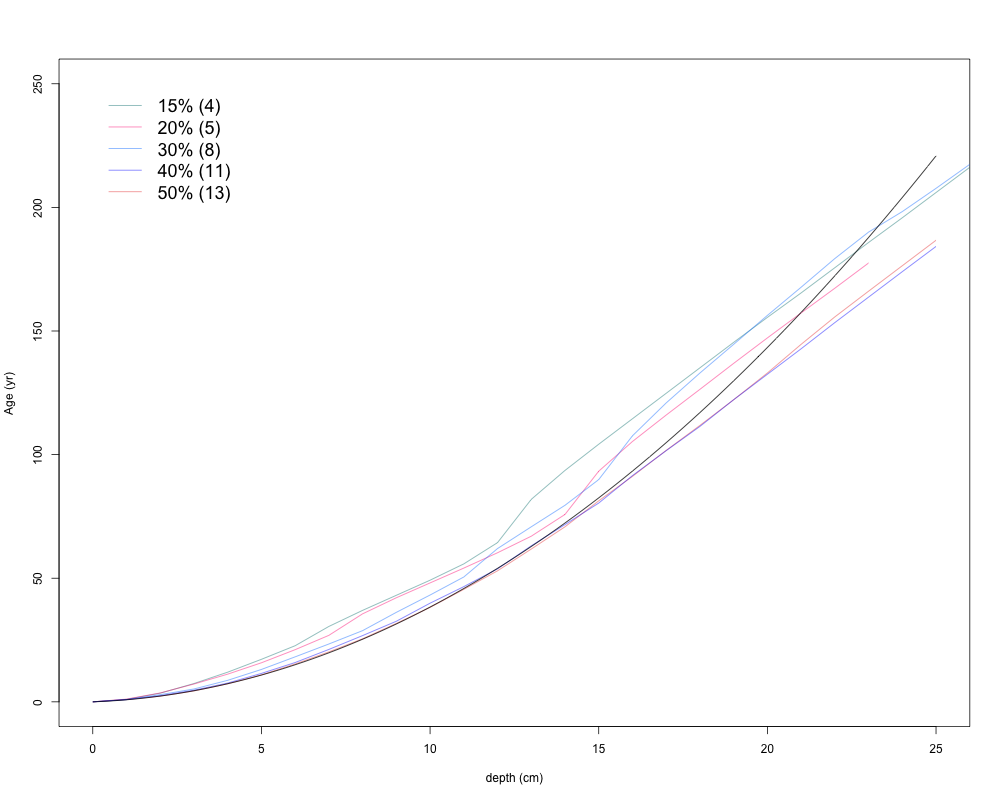
\includegraphics[width=10cm]{./Figures/Chrono_ssize.png}
			\caption{}
			\label{}
		\end{centering}
	\end{figure}
\end{frame} 


\begin{frame}{Aprendizaje (muestreo)}
 	\begin{figure}
		\begin{centering}
			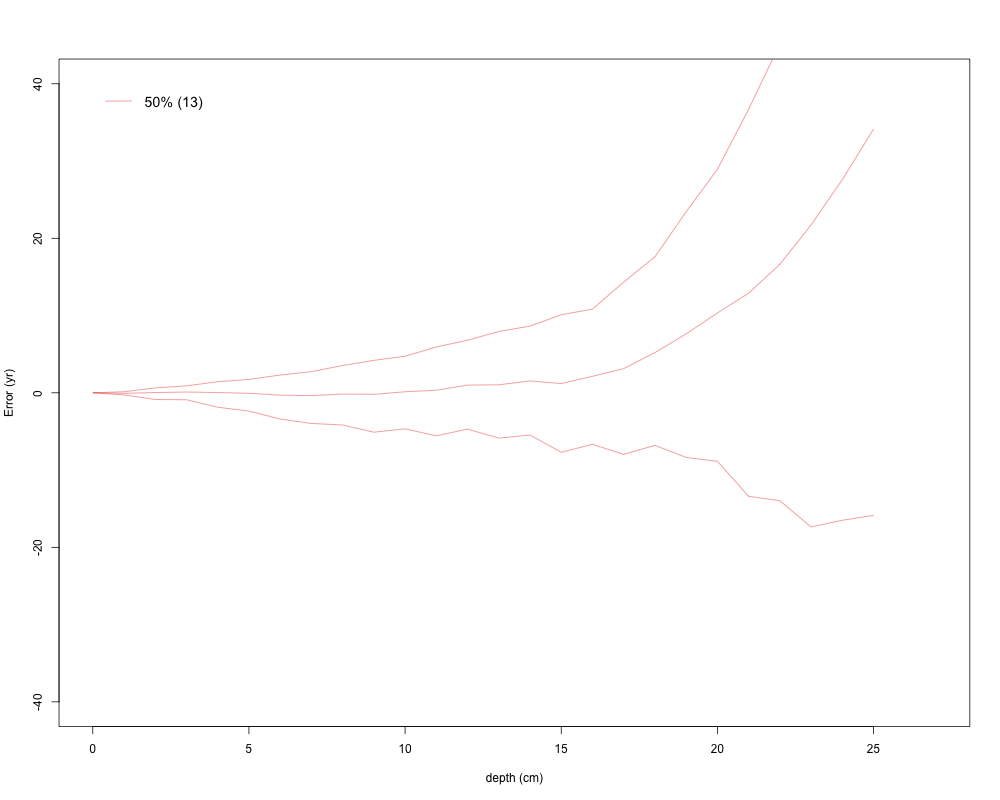
\includegraphics[width=10cm]{./Figures/Chrono_ssize_difsd50.png}
			\caption{}
			\label{}
		\end{centering}
	\end{figure}
\end{frame} 

\begin{frame}{Aprendizaje (muestreo)}
 	\begin{figure}
		\begin{centering}
			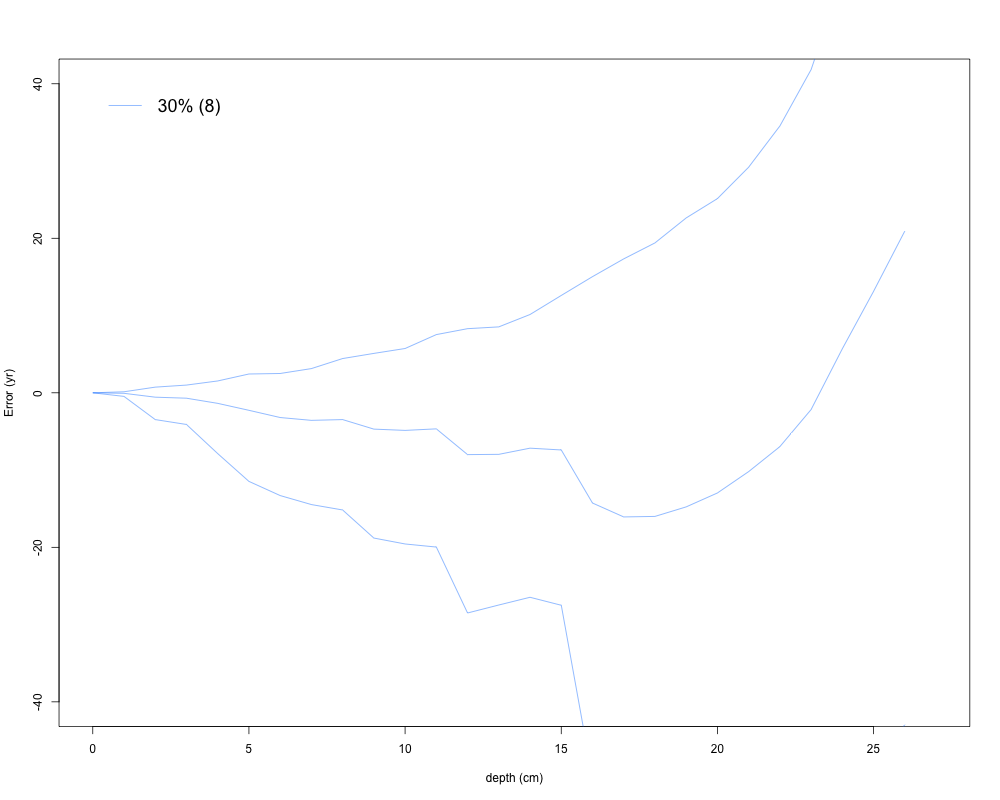
\includegraphics[width=10cm]{./Figures/Chrono_ssize_difsd30.png}
			\caption{}
			\label{}
		\end{centering}
	\end{figure}
\end{frame} 


\begin{frame}{Aprendizaje (muestreo)}
 	\begin{figure}
		\begin{centering}
			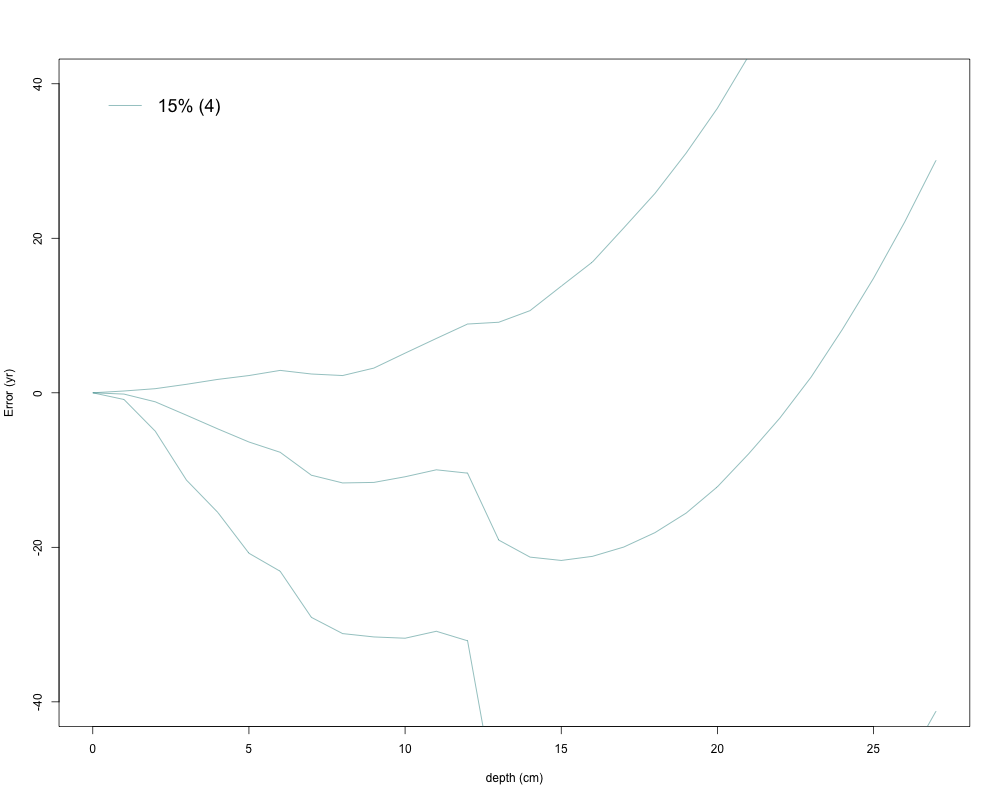
\includegraphics[width=10cm]{./Figures/Chrono_ssize_difsd10.png}
			\caption{}
			\label{}
		\end{centering}
	\end{figure}
\end{frame} 


\begin{frame}{Aprendizaje (muestreo)}
 	\begin{figure}
		\begin{centering}
			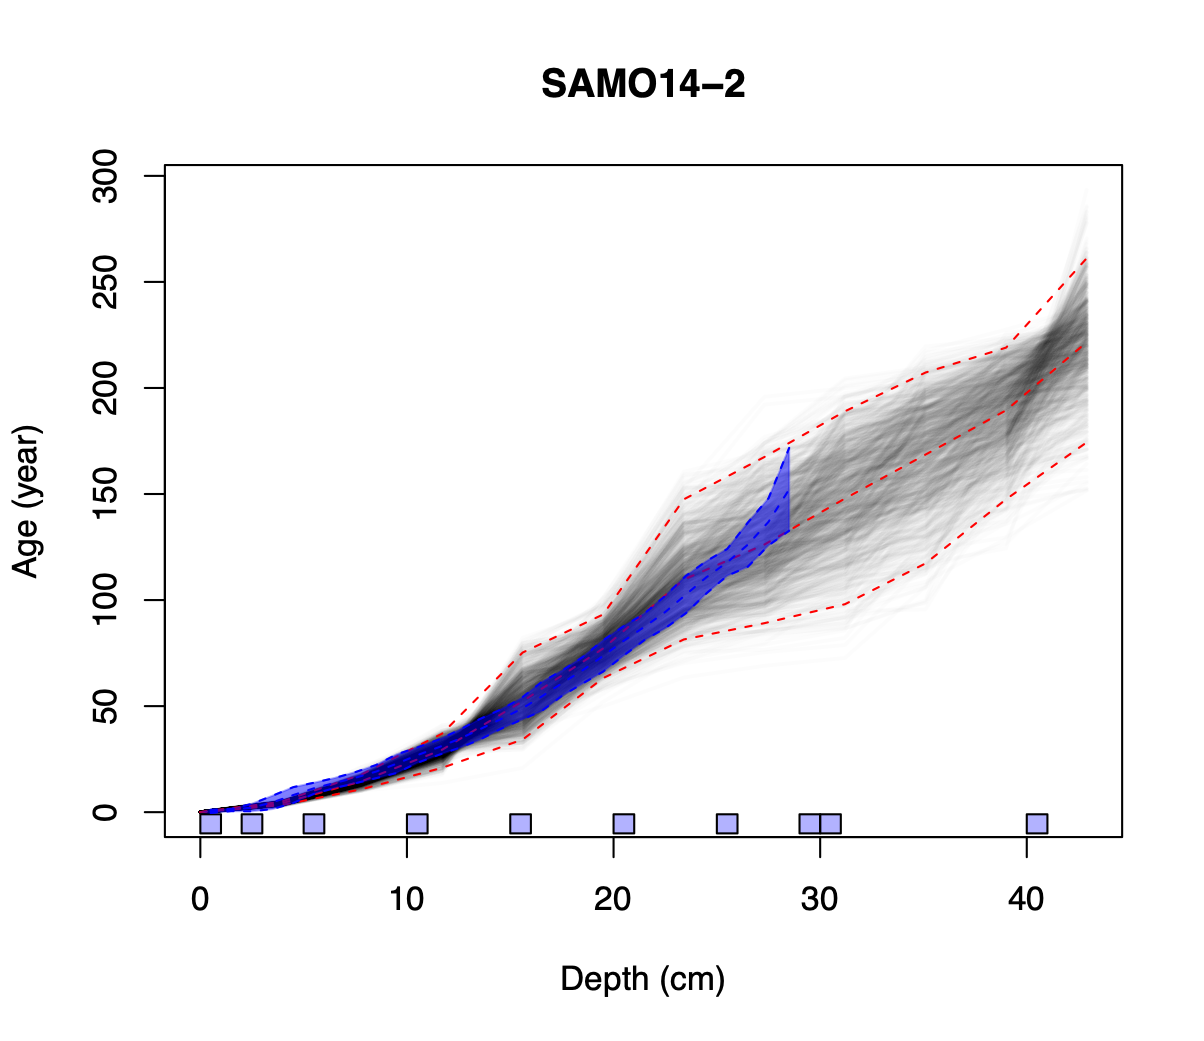
\includegraphics[width=10cm]{./Figures/SAMO14_2.png}
			\caption{}
			\label{}
		\end{centering}
	\end{figure}
\end{frame} 

\begin{frame}{Aprendizaje (muestreo)}
 	\begin{figure}
		\begin{centering}
			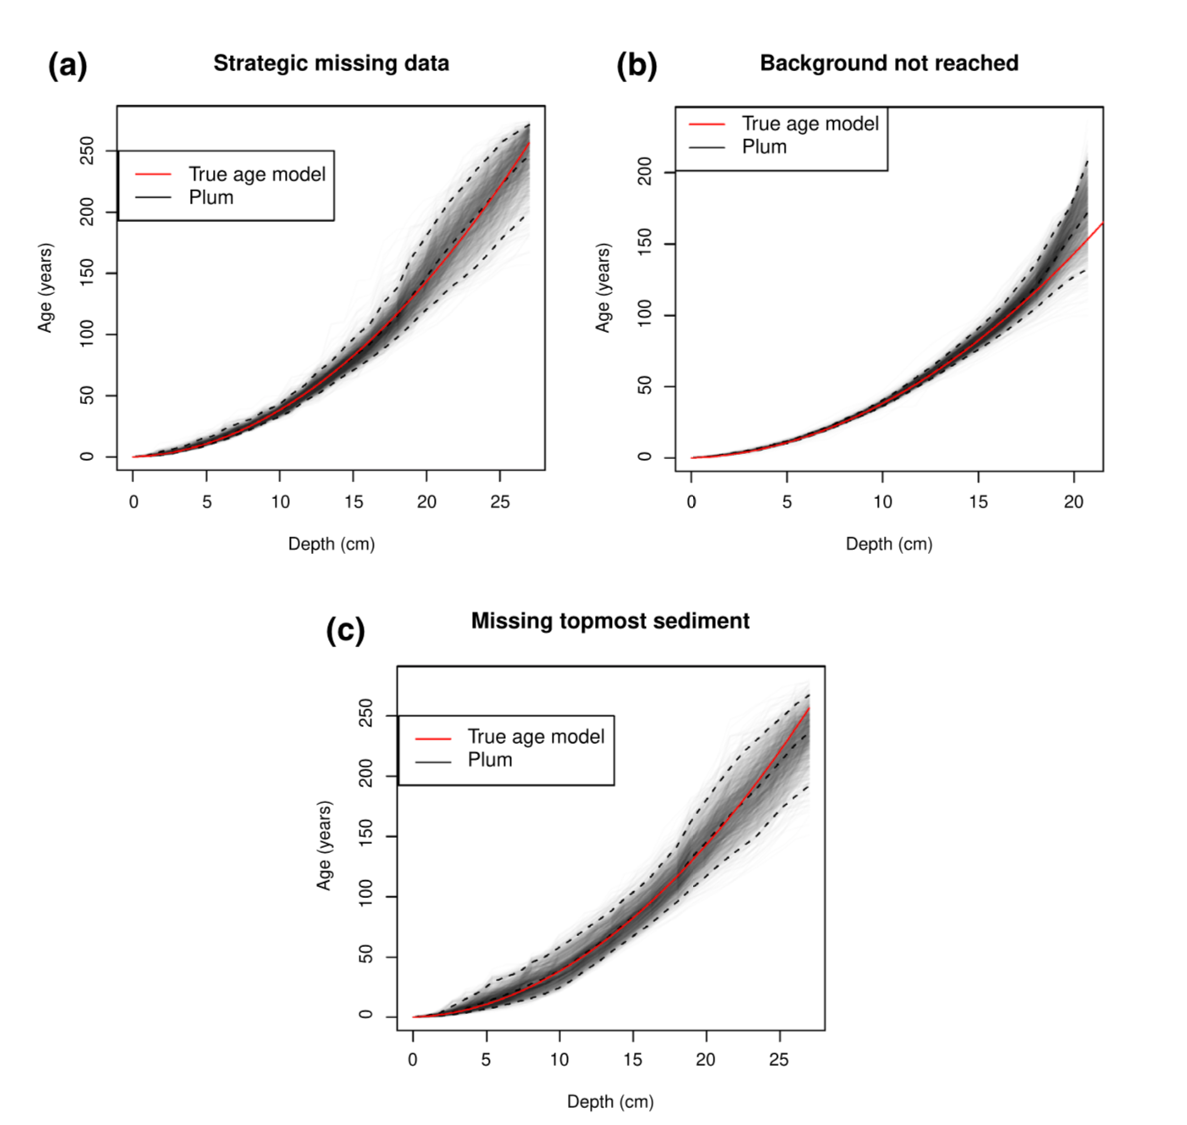
\includegraphics[width=8.5cm]{./Figures/Simulation_paper.png}
			\caption{}
			\label{}
		\end{centering}
	\end{figure}
\end{frame} 



\begin{frame}{Otros fechamientos}
	\begin{block}{$^{137}$Cs}
		En el caso de $^{137}$Cs, la incorporación de esta información se hace a través de la función de verosimilitud.
		\begin{eqnarray}
			\mathcal{L}\left(\Theta\right) = \mathcal{L}_{^{210}Pb}\left(\Theta\right) \mathcal{L}_{^{137}Cs}\left(\Theta\right).
		\end{eqnarray}
	\end{block} 
\end{frame}

\begin{frame}{Otros fechamientos}
	\begin{figure}
		\begin{centering}
			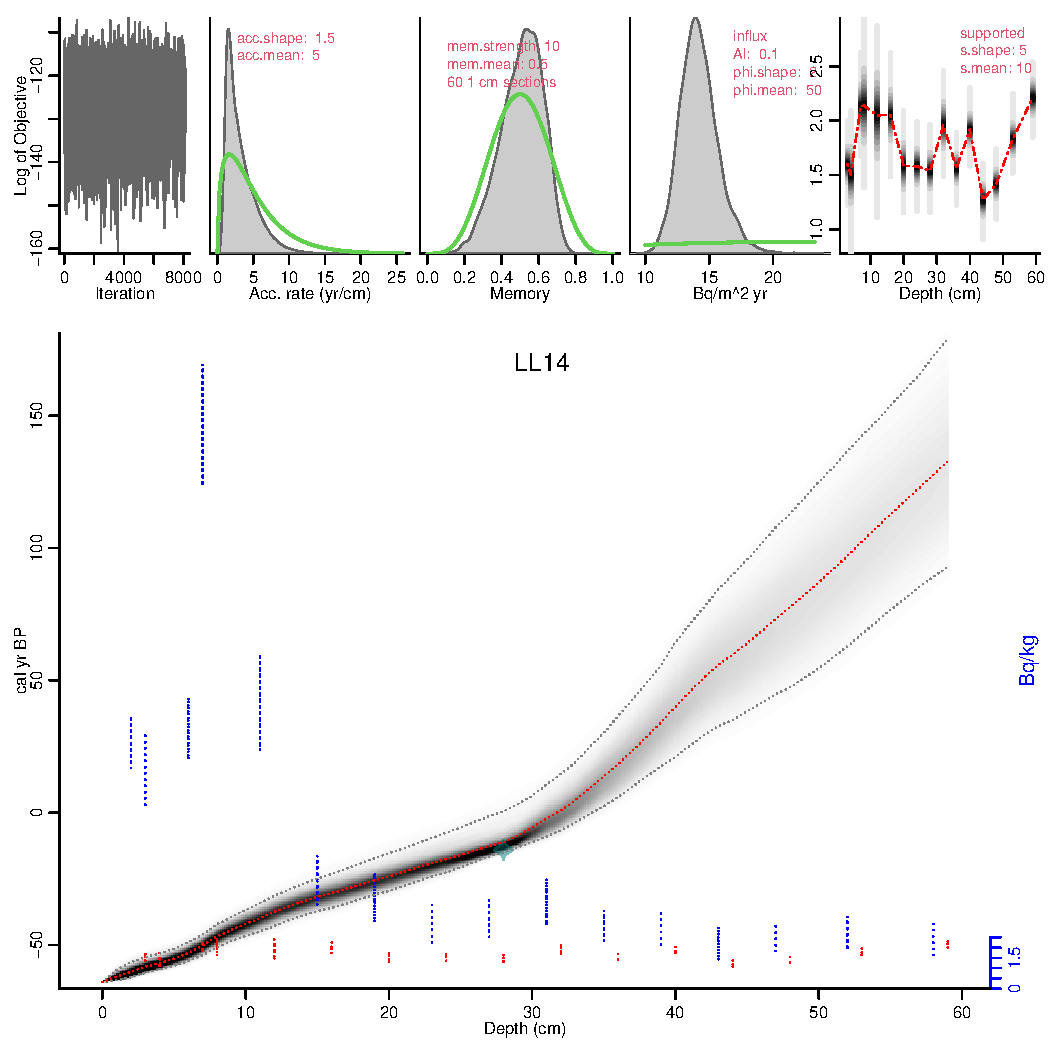
\includegraphics[width=8cm]{./Figures/LL14_60.pdf}
			\caption{}
			\label{}
		\end{centering}
	\end{figure}
\end{frame} 


\begin{frame}{otros fechamientos}
	\begin{block}{$^{14}$C }
		\begin{eqnarray}
			\mathcal{L}\left(\Theta\right) = \mathcal{L}_{^{210}Pb}\left(\Theta\right)\mathcal{L}_{^{14}C}\left(\Theta\right) \mathcal{L}_{^{137}Cs}\left(\Theta\right).
		\end{eqnarray}
	\end{block} 
\end{frame} 

\begin{frame}{Otros fechamientos }
	\begin{figure}
		\begin{centering}
			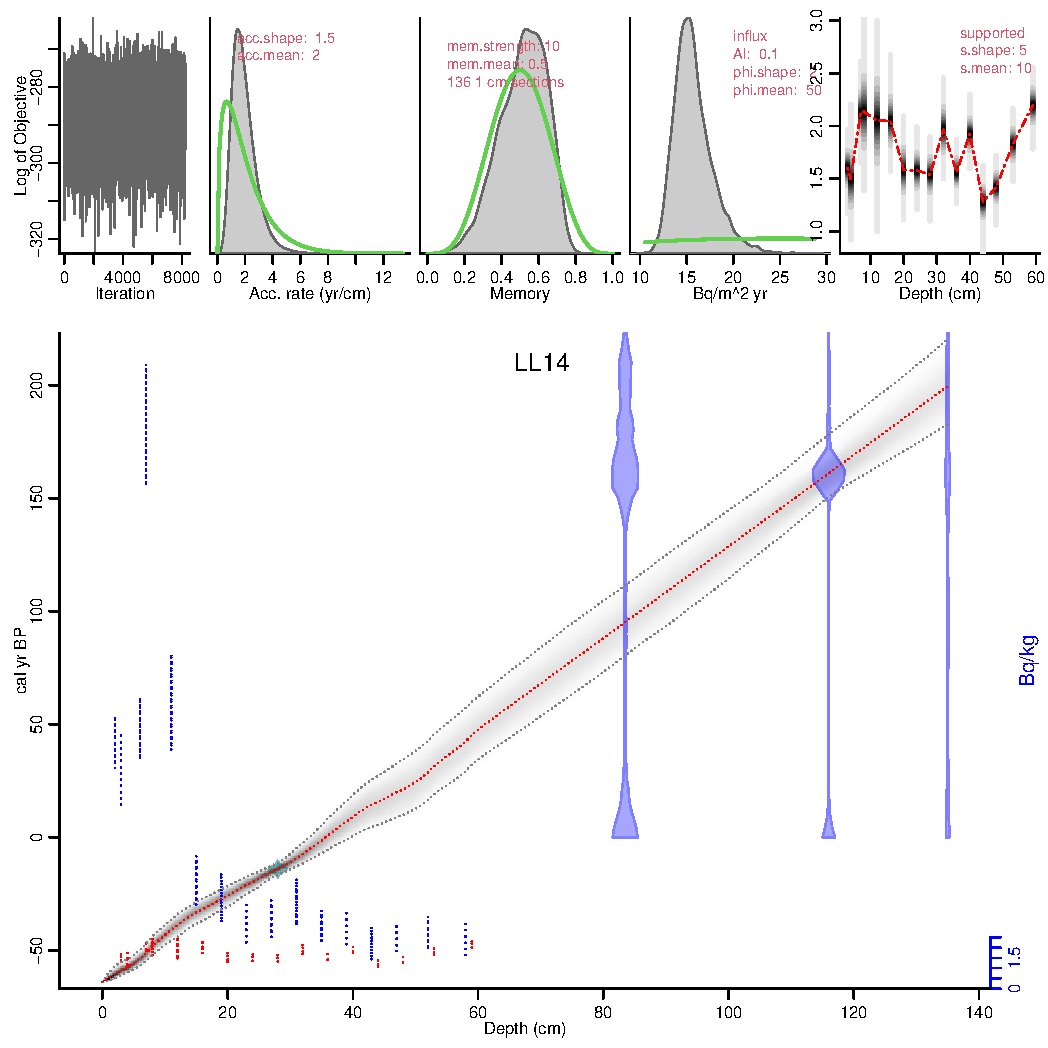
\includegraphics[width=8cm]{./Figures/LL14_136.pdf}
			\caption{}
			\label{}
		\end{centering}
	\end{figure}
\end{frame} 


\begin{frame}{Gracias}
	GRACIAS
\end{frame} 




\end{document}
